\documentclass[a4paper,oneside,12pt]{article}
\usepackage[slovene]{babel}
\usepackage[utf8]{inputenc}
\usepackage{url}
\usepackage{graphicx}
\usepackage{epstopdf}
\usepackage[usenames]{color}
\usepackage[reqno]{amsmath}
\usepackage{amssymb}
\usepackage{fancybox}
\usepackage{listings}
\usepackage{wasysym}
\usepackage[bookmarks, colorlinks=true, %
linkcolor=black, anchorcolor=black, citecolor=black, filecolor=black,%
menucolor=black, runcolor=black, urlcolor=black%
]{hyperref}
\hypersetup{pdftitle={Iskanje optimalnega splošnega kompozitnega sortirnega algoritma}}
\hypersetup{pdfauthor={Jure Slak}}
\hypersetup{pdfsubject={Raziskovalna naloga}}
\usepackage[
    paper=a4paper,
    top=2.5cm,
    bottom=2.5cm,
%    textheight=24cm,
    textwidth=15cm,
    ]{geometry}


\usepackage{amsthm}
{
\newtheorem{izrek}{Izrek}[section]
\newtheorem{lema}[izrek]{Lema}
\newtheorem{trditev}[izrek]{Trditev}
\newtheorem{posledica}[izrek]{Posledica}
{
\theoremstyle{definition}
\newtheorem{definicija}{Definicija}
}
}


\def\R{\mathbb R}
\def\N{\mathbb N}
\def\Z{\mathbb Z}
\def\C{\mathbb C}
\def\Q{\mathbb Q}
\def\ali{\;|\;}
\mathchardef\mhyphen="2D

\usepackage{algorithm}
\usepackage{algpseudocode}

\algnewcommand\algorithmicto{\textbf{to}}
\algnewcommand\algorithmicswap{\textsc{swap}}
\algnewcommand\Swap[2]{\State \ensuremath{\algorithmicswap(#1,\ #2)}}
\algrenewtext{For}[3]{$\algorithmicfor\ #1 \gets #2\ \algorithmicto\ #3\ \algorithmicdo$}

\newenvironment{BNF}{
    \\
    \Sbox
    \minipage{12cm}
}{
    \endminipage
    \endSbox
    \minipage{\textwidth}
    \vspace*{5pt}
    \begin{center}
        \fcolorbox{white}{white}{
            \TheSbox
        }
    \end{center}
    \vspace*{5pt}
    \endminipage
}

\def\:{\,::=\,}
\def\bnfassign:{\,::=&\,}
\def\para{\ensuremath{\,|\,}}
\newcommand{\q}[1]{\text{``}#1\text{''}}
\newcommand{\ntm}[1]{\ensuremath{<\!\!\text{#1}\!\!>}}
\newcommand{\bnf}[2]{\ensuremath{\ntm{#1} \: #2}}
\newcommand{\abnf}[2]{\ensuremath{\ntm{#1} \bnfassign: #2}}
\newcommand{\konfarrow}{\mbox{--}~\mbox{--}~\mbox{\ensuremath{>}}}
\newcommand{\lra}{\ensuremath{\longrightarrow}}
\newcommand{\subsubsubsection}[1]{\vspace*{1ex}\textbf{#1}\\}

\floatname{algorithm}{Algoritem}

% your definitions here ... 

\title{Iskanje optimalnega splošnega kompozitnega sortirnega algoritma}
\author{Jure Slak}
\date{\today}

\begin{document}

\renewcommand{\listfigurename}{Kazalo slik} 
\renewcommand{\listalgorithmname}{Kazalo algoritmov}

\addto\captionsslovene { %
\renewcommand\bibname{} %
}
\renewcommand\refname{}

\lstset{language=c++, morekeywords={function, swap, to, conf_t, container_t, size_t,
cmp_t, RAI}}

\thispagestyle{empty}

\begin{center}{\large
  Gimnazija Vič
  \vfill
  {\Large Jure Slak}\\[20mm]
  {\bf \huge Iskanje optimalnega splošnega kompozitnega sortirnega algoritma}\\[10mm]
  Raziskovalna naloga\\[1cm]
  Mentor: prof. Klemen Bajec \\[2mm]
  Mentor: Gašper Ažman, dipl. mat.}
  \vfill
  \vfill
  \large Ljubljana, 2011
\end{center}
\pagebreak

\thispagestyle{empty}
\tableofcontents
\pagebreak
\thispagestyle{empty}
\listoffigures
\pagebreak
\thispagestyle{empty}
\listofalgorithms
\pagebreak

\section{Uvod}
\label{chapter:uvod}

Sortiranje ali urejanje na splošno pomeni preurejanje dane množice objektov
v nek določen vrstni red.
Namen sortiranja je ponavadi olajšati kasnejše iskanje pripadnikov take urejene množice. Kot tako je
v vsesplošni uporabi in ima velik pomen. Objekti so sortirani v telefonskih imenikih,
davčnih registrih, stvarnih kazalih, knjižnicah, slovarjih, skladiščih in skoraj povsod tam,
kjer moramo shranjene predmete iskati in dosegati. Že majhne otroke učimo, da stvari spravljajo
``v red'' in tako z neke vrste sortiranjem prihajajo v stik daleč preden se naučijo kaj
aritmetike.

\subsection{Teoretični uvod}
\label{chapter:teoreticni}
Sortiranje je torej pogosto in pomembno opravilo in tudi zaradi tega se je je skozi čas
razvilo veliko različnih postopkov za čimbolj učinkovito urejanje. Eden izmed razlogov za
veliko število postopkov je tudi ta, da ima prav vsak od njih neko prednost pred ostalimi in je
zaradi tega v določenih primerih boljši od ostalih. V nadaljevanju bom opisal nekaj najbolj znanih, 
vendar jih obstaja še mnogo več. 

\subsubsection{Definicija algoritma}

\textbf{Algoritem} je končno zaporedje ukazov, ki, če jih ubogamo, opravijo neko nalogo.
Zanj velja:
\begin{itemize}
  \item \textbf{Ima podatke}. Množica podatkov je lahko tudi prazna.
  \item \textbf{Vrne rezultat}. Vrne vsaj eno izračunano vrednost ali kaj stori, kot na primer
    premakne papir na tiskalniku na novo stran.
  \item \textbf{Je natančno določen}. Vsak ukaz mora nedvoumno povedati kaj storiti.
  \item \textbf{Se vedno konča}. Končati se mora pri vseh možnih naborih vhodnih podatkov.
  \item \textbf{Mogoče ga je opraviti}. V načelu ga je mogoče izpeljati ``peš'', s papirjem in
    svinčnikom.
\end{itemize}
% citat [KOZ86], str 11

% zakaj je 1.1. namesto 1
\begin{definicija}
  Algoritem je \textbf{kompoziten} oziroma \textbf{sestavljen}, če je sestavljen iz večih
  drugih algoritmov.
\end{definicija}


\subsubsection{Definicija sortiranja}
\label{chapter:sortdef}
Naj bo dan končen vektor elementov $\vec{a} \in A$, linearno urejena množica ključev $(K,
\leq)$ in funkcija $f\!\!: A \rightarrow K, f\!\!: a \mapsto k$\footnote{
$f$ je ponavadi trivialen, ker je $f(a)$ ponavadi kar del
$a$-ja in nam ga ni treba računati, lahko pa to ni res.}, ki vsakemu $a \in A$ priredi
njegov ključ $k \in K$.
Tedaj lahko definiramo relacijo linearne urejenosti $\leq$ med elementi $A$.
\[ a \leq a' \overset{\text{def}}{\Longleftrightarrow} f(a) \leq f(a') \hspace{3em} \forall\ a, a' \in A \]


Sortiranje pomeni permutiranje elementov vektorja $\vec{a}$ tako, da velja:
\[ a_1 \leq a_2 \leq \cdots \leq a_n.\]

Definirajmo še tip \emph{item}, ki naj ponazarja elemente $\vec{a}$-ja. Naj bo \emph{key}
ključ elementa tipa \emph{cmp\_t}, na katerem je definirana relacija linearne urejenosti.

\begin{lstlisting}
struct item {
    cmp_t key;
    /* ostale komponente */
};
\end{lstlisting}

Ostale komponente predstavljajo s stališča urejanja nepomembne podatke o elementih v
polju.
S stališča sortirnih algoritmov je ključ torej \emph{edini} pomemben podatek in zato
ostalih komponent ni treba podrobno definirati.

\begin{definicija}
  \textbf{Sortirni algoritem} je algoritem, ki prejme neko podatkovno strukturo s podatki
  in neko relacijo linearne urejenosti med njimi ter jih uredi po vrstnem redu, ki ga določa ta
  relacija.
\end{definicija}

\begin{definicija}
  Za sortirni algoritem pravimo, da je \textbf{stabilen}, če ostane po končanem sortiranju
  relativni vrstni red elementov z istim ključem nespremenjen.
  Stabilnost sortiranja je pogosto zaželena, če so elementi že urejeni po neki
  sekundarni $\leq$ relaciji, torej glede lastnosti, ki je (primarni) ključ ne izraža.
\end{definicija}

\begin{definicija}
  O neki sortirni metodi pravimo, da se dogaja \textbf{na mestu}, če se med izvajanjem podatki, ki
  jih sortiramo, ne kopirajo v dodaten pomnilnik.
\end{definicija}

\begin{definicija}
  Sortirni algoritem je \textbf{primerjalen}, če ureja elemente tako, da jih primerja med seboj.
\end{definicija}


Vsi nadaljnji algoritmi bodo definirani kot procedure s tremi parametri, $a$, $prvi$,
$zadnji$, ki predstavljajo:
\begin{itemize}
  \item $a$: polje, ki ga sortiramo. V splošnem zahtevamo, da je to katerakoli podatkovna
    struktura, ki podpira neko vrsto naključnega dostopa. Le-tega uporabljamo, kadar 
    uporabljamo operator $[\cdot]$. Zaradi časovne analize algoritmov zahtevamo, da operator 
    $[\cdot]$ deluje v konstantnem času. Indeksiranje elementov polja se začne z 0.
    V nadaljnjem opisovanju bom uporabljal besedo
    \textbf{polje} za katerokoli podatkovno strukturo, ki ustreza zgornjim zahtevam.
  \item $prvi$: indeks prvega elementa, ki ga želimo sortirati.
  \item $zadnji$: indeks elementa, ki je \emph{za} zadnjim elementom, ki ga sortiramo. Lahko ni
    veljaven indeks v $a$.
\end{itemize}
Vse procedure bodo spremenile polje $a$, nobena ne bo ničesar vrnila.

Pri definiciji časovne in prostorske zahtevnosti algoritma bo za prostorsko zahtevnost 
navedena zgolj dodatna poraba pomnilnika, saj vsi algoritmi porabijo $O(n)$ pomnilnika za
shranjevanje celotnega polja, kjer $n$ predstavlja število elementov v polju, ali razliko
$zadnji - prvi$. 

%% poravnava
\subsubsection{Rekurzija}
\label{chapter:rekurzija}
Rekurzija je proces ponavljanja elementov na nek samopodoben način. V matematiki in 
računalništvu se nanaša na način definiranja funkcij. Rekurzivna funkcija je tista, 
ki se v svoji definiciji sklicuje sama nase. Če želimo da je taka definicija sploh 
smiselna, moramo podati vsaj en osnoven nerekurziven primer in še množico pravil, 
ki vse ostale primere prevedejo v osnovni primer.

Poglejmo si primer definicije fakultete\footnote{Bolj običajno se fakulteto definira kot:
$n! = \displaystyle\prod_{k=1}^{n} k = 1 \cdot 2 \cdot 3 \cdot \ \cdots\  \cdot n$}. Fakulteta naravnega števila $n$ je v matematiki
funkcija, ki določa zmnožek vseh celih števil, manjših ali enakih $n$. Označi se jo z $n!$.
\[
n! = \left\{ 
\begin{array}{rl}
     1             & \mbox{;če $n = 1$} \\
     n \cdot (n-1)!& \mbox{;sicer}
\end{array} \right.
\]
Pri fakulteti imamo definiran en osnovni primer ($1! = 1$), vsi ostali primeri pa se prej
ali slej pretvorijo v ta primer. Poglejmo si primer števila 4.
\begin{enumerate}
  \item Ker 4 ni enako 1, gledamo drugo pravilo za izračun fakultete: $4!$ je torej $4
    \cdot (4 - 1)!$
  \item V izračunu imamo še vedno fakulteto, torej pogledamo kako se izračuna $3!$, da
    lahko izračunamo $4 \cdot 3!$.
  \item 3 ni enako 1, torej gledamo drugo pravilo, $3! = 3 \cdot 2!$. Iz tega sledi $4! =
    4 \cdot 3 \cdot 2!$. V računu nastopa $2!$, izračunamo jo po drugem pravilu.
  \item $2!$ izračunamo kot $2 \cdot 1!$, $4! = 4 \cdot 3 \cdot 2 \cdot 1!$. V računu še
    vedno nastopa fakulteta, torej jo izračunamo.
  \item $1!$ je po prvem pravilu enaka $1$. $4!$ smo prevedli v $4 \cdot 3 \cdot 2 \cdot
    1$. Zdaj lahko brez problemov izračunamo $4!$.
  \item Zmnožimo in dobimo rezultat $4! = 24$.
\end{enumerate}
\subsubsection{Psevdokoda}
Psevdokoda je neformalen zapis nekega algoritma, ki uporablja strukture iz programskih
jezikov in je pomensko pravilen, namenjen predvsem lažjemu razumevanju algoritma.

Pri opisu algoritmov v psevdokodi bom uporabljal prireditve (označene s $\gets$), 
\textbf{while} zanke, \textbf{for} zanke, vejitve (\textbf{if} stavke), klice 
funkcij in osnovne  matematične ($+, -, \cdot, /$) in logične operatorje ($=, 
\neq, \wedge, \vee, \neg, <, \leq, >, \geq$) ter oklepaje ($(), \lfloor\rfloor$). 
Za polja $a[i]$ pomeni element polja na indeksu $i$, polja se začnejo z indeksom $0$.
Predpostavil bom tudi da že obstaja funkcija \textbf{swap}, ki zamenja vrednosti dveh
spremenljivk.

\subsubsection{Urejanje z navadnim vstavljanjem}
\label{chapter:insertionsort}
Urejanje z navadnim vstavljanjem (\emph{angl.} insertion sort) je metoda,
podobna tisti, ki jo na široko uporabljajo igralci kart. Je primerjalni sortirni algoritem.

Zaporedje $a_1, a_2, \ldots, a_n$ razdelimo na že urejeni del $a_1, a_2, \ldots, a_{i-1}$
in še neurejeni del $a_i, \ldots a_n$. Na vsakem koraku, začenši z $i = 2$ in
prirastkom ena, vstavimo $i$-ti element začetnega zaporedja na ustrezno mesto v končnem
zaporedju. Ko je $i$ enak 2, je prvi del trivialno sortiran, saj vsebuje le en element.

\begin{figure}[h]
    \begin{center}
        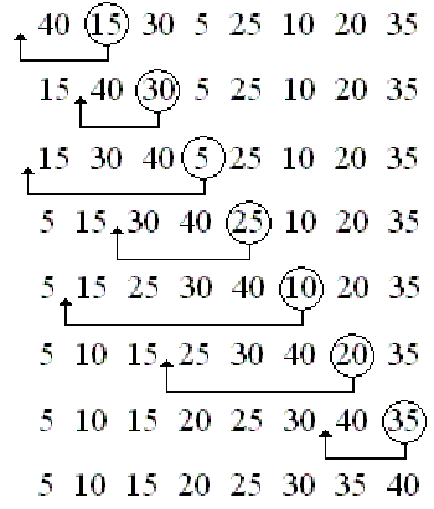
\includegraphics[height=45mm]{slike/insertionsort.png}
    \end{center}
    \vspace{-0.7cm}
    \caption[Urejanje z vstavljanjem]{Grafična predstavitev urejanja z navadnim vstavljanjem.}
    \label{fig:insertionsortimage}
\end{figure}

Na sliki \ref{fig:insertionsortimage} je prikazan postopek sortiranja z navadnim vstavljanjem na primeru osmih naključno
izbranih števil. Algoritem navadnega
vstavljanja je v psevdokodi napisan kot algoritem \ref{algo:insertionsort}.

\begin{algorithm}
  \caption{Urejanje z vstavljanjem}\label{algo:insertionsort}
  \begin{algorithmic}[1]
    \Function{insertionsort}{a, prvi, zadnji}
        \For{i}{prvi + 1}{zadnji}
            \State $x \gets a[i]$
            \State $j \gets i - 1$
            \While{$x < a[j] \wedge j \geq 0$}
                \State $a[j+1] \gets a[j]$
                \State $j \gets j - 1$
            \EndWhile
            \State $a[j+1] \gets x$
        \EndFor
    \EndFunction
  \end{algorithmic}
\end{algorithm}

Med postopkom iskanja pravega mesta je dobro sproti premikati elemente med izvajanji
primerjanj. Z drugimi besedami, pustiti $x$, da se ``pogrezne'' tako, da $x$
primerjamo z naslednjim elementom $a_j$ in ga bodisi vstavimo, če je ključ $a_j$ manjši
ali enak $x$ ali pa $a_j$ premaknemo na desno ter nadaljujemo proti levi, če še nismo pri
levem robu polja. Postopek ``pogrezanja'' lahko ustavita ta dva ločena
pogoja, kot je prikazano v zgornji \emph{while} zanki.  Ko vstavimo še zadnji element v že 
urejeno zaporedje, smo z urejanjem zaključili.

\subsubsubsection{Časovna in prostorska zahtevnost}
Časovna zahtevnost je v 
\begin{itemize}
  \item najboljšem primeru $O(n)$
  \item povprečnem primeru $O(n^2)$
  \item najslabšem primeru $O(n^2)$
\end{itemize}

Prostorska zahtevnost je v vsakem primeru $O(1)$, saj se vse premene dogajajo na
mestu.\\

Spodnja časovna meja ustreza primeru, ko so elementi na začetku že urejeni, zgornja pa primeru,
ko so elementi na začetku nasprotno urejeni. Podani algoritem opisuje tudi stabilen postopek sortiranja, kajti medsebojni
vrstni red elementov z enakimi ključi ostane nespremenjen.

Urejanje z navadnim vstavljanjem je zelo učinkovito na majhnih poljih. Učinkovito je tudi na že
skoraj sortiranih poljih, saj se s tem približujemo obnašanju v najboljšem primeru.
Zaradi kvadratne časovne zahtevnosti je urejanje z navadnim vstavljanjem zelo neučinkovito na
dolgih poljih, če ta niso že skoraj urejena.

\subsubsection{Urejanje z izbiranjem}
\label{chapter:selectionsort}
Urejanje z izbiranjem (\emph{angl.} selection sort) je eden najenostavnejših primerjalnih sortirnih
algoritmov.

Algoritem je sledeč:
\begin{enumerate}
  \item najdi element z najmanjšim ključem
  \item zamenjaj ga s prvim elementom
  \item ponovi zgornja koraka za ostanek polja.
\end{enumerate}

Polje je med sortiranjem razdeljeno na dva dela: podpolje že urejenih elementov, ki se
nahaja na začetku in podpolje elementov, ki jih je še potrebno sortirati in zasedajo
preostali del polja.

Postopek urejanja z izbiranjem je prikazan na sliki \ref{fig:selectionsortimage}.
Najmanjši elementi v drugem delu polja so obkroženi, puščica ponazarja, kako jih
vstavimo na konec prvega dela. Dela sta ločena z dvopičjem. % ne še

\begin{figure}[h]
    \begin{center}
        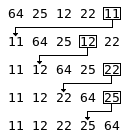
\includegraphics[height=40mm]{slike/selectionsort.png}
    \end{center}
    \vspace{-0.7cm}
    \caption[Urejanje z izbiranjem]{Grafična predstavitev urejanja z navadnim vstavljanjem.}
    \label{fig:selectionsortimage}
\end{figure}

V psevdokodi je urejanje z izbiranjem zapisano kot algoritem \ref{algo:selectionsort}.

\begin{algorithm}
  \caption{Urejanje z izbiranjem}\label{algo:selectionsort}
  \begin{algorithmic}[1]
    \Function{selectionsort}{a, prvi, zadnji}
        \For{i}{prvi}{zadnji}
            \State $x \gets i$
            \For{j}{i + 1}{zadnji}
                \If{$a[j] < a[x]$}
                    \State $x \gets j$
                \EndIf
            \EndFor
            \Swap{a[x]}{a[i]}
        \EndFor
    \EndFunction
  \end{algorithmic}
\end{algorithm}

\subsubsubsection{Časovna in prostorska zahtevnost}
Časovna zahtevnost je v vsakem primeru enaka in sicer $O(n^2)$.

Prostorska zahtevnost je v najboljšem, povprečnem in najslabšem primeru $O(1)$, 
saj algoritem opravlja vse premene na mestu.

Ker ima urejanje z izbiranjem v vsakem primeru kvadratno časovno zahtevnost, je neprimerno
za daljša polja. Urejanje z izbiranjem tudi ni odvisno od prvotnega vrstnega reda,
saj mora za iskanje najmanjšega elementa vedno pregledati celoten ostanek polja.
Njegova prednost je v tem, da stori zelo malo zamenjav elementov, kar je še posebej
primerno takrat, ko je premikanje elementov drago (imamo velike elemente).

\subsubsection{Hitro urejanje}
\label{chapter:quicksort}
Hitro urejanje ali urejanje s porazdelitvami\footnote{vir: IJS-jev slovar računalniških izrazov
\url{http://www.ijs.si/cgi-bin/rac-slovar}}(\emph{angl.} quicksort) je eden izmed
najučinkovitejših sortirnih algoritmov, ki jih poznamo, razvil pa ga je C. A. R. Hoare.
Je primerjalni sortirni algoritem, ki je zgrajen na principu deli in vladaj.

Sortiranje s porazdelitvami temelji na dejstvu, da moramo premene opravljati na večje
razdalje, da bi bile učinkovitejše. Recimo, da imamo $n$ nasprotno urejenih elementov.
V tem primeru jih lahko sortiramo z le $^n/_2$ premenami tako, da najprej premenjamo prvega
in zadnjega in se postopoma pomikamo proti sredini. Seveda je to možno le, če vemo, da so 
elementi natanko nasprotno urejeni.

Prejšnji primer nas napelje na naslednji algoritem: 
izberemo poljuben element (recimo mu pivot in ga označimo z $x$), nato začnemo 
polje $a$ pregledovati z leve, dokler ne najdemo elementa $a_i > x$ in nato z desne dokler ne 
najdemo elementa $a_i < x$. Elementa sedaj medsebojno zamenjamo in nadaljujemo s 
pregledovanjem in premenami, dokler se ne srečamo nekje na sredi polja.
Polje je sedaj razdeljeno na levi del s ključi manjšimi od $x$ in na desni del
s ključi večjimi od $x$. Pivot nato umestimo med oba dela, kar je tudi njegovo končno
mesto in metodo ponovimo na delih levo in desno od pivota dokler ne pridemo do že urejenih
podpolj, torej tistih z dolžino manjšo ali enako 1. 

Iz prejšnjega algoritma ugotovimo, da je izbira pivota zelo
pomembna. Pogosto je, da za pivot vzamemo kar zadnji element, vendar to sproži ravno
najslabšo možnost izvajanja programa, če so elementi že urejeni. Zato sem v svoji
implementaciji za pivot vzel mediano prvega, srednjega in zadnjega elementa oziroma t.i.
mediano treh. Pogosta izbira je tudi naključni pivot. 

Postopek sortiranja s porazdelitvami je prikazan na primeru devetih naključno
izbranih števil (glej sliko \ref{fig:quicksortimage}). Izbrani pivoti so obarvani sivo.
Vsaka vrstica predstavlja svojo globino rekurzije.

\begin{figure}[h]
    \begin{center}
        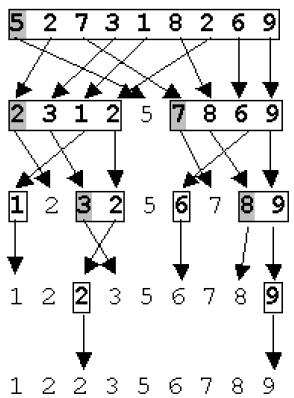
\includegraphics[height=45mm]{slike/quicksort.jpg}
    \end{center}
    \vspace{-0.7cm}
    \caption[Hitro urejanje]{Grafična predstavitev urejanja s porazdelitvami.}
    \label{fig:quicksortimage}
\end{figure}

V psevdokodi je algoritem hitrega urejanja zapisan kot algoritem \ref{algo:quicksort}.

\begin{algorithm}
  \caption{Hitro urejanje}\label{algo:quicksort}
  \begin{algorithmic}[1]
    \Function{quicksort}{a, prvi, zadnji}
        \If{$zadnji - prvi < 2$} \Return \EndIf
        \State $s \gets first$
        \State $e \gets last - 1$
        \State $m \gets \lfloor(s+e)/2\rfloor$
        \If{$a[m] < a[s] < a[e] \vee a[e] < a[s] < a[m]$}
            \Swap{a[s]}{a[e]}
            \Comment{a[s] je mediana treh}
        \ElsIf{$a[e] < a[m] < a[s] \vee a[s] < a[m] < a[e]$}
            \Swap{a[m]}{a[e]}
            \Comment{a[m] je mediana treh}
        \EndIf

        \State $pivot \gets a[e]$
        \State $e \gets e - 1$

        \While{$s \leq e$}
            \While{$s \leq e \wedge a[s] < pivot$}
                \Comment{prvi element z leve, ki je večji od pivota}
                \State $s \gets s + 1$
            \EndWhile
            \While{$s \leq e \wedge \neg(a[e] < pivot)$}
                \Comment{prvi element z desne, ki je manjši od pivota}
                \State $e \gets e - 1$
            \EndWhile
            \If{$s < e$}
                \Swap{a[s]}{a[e]}
            \EndIf
        \EndWhile
        \State $a[zadnji - 1] \gets a[s]$
        \State $a[s] \gets pivot$
        \State \textsc{quicksort}$(a, prvi, s)$
        \State \textsc{quicksort}$(a, s + 1, zadnji)$
    \EndFunction
  \end{algorithmic}
\end{algorithm}

\subsubsubsection{Časovna in prostorska zahtevnost}
Časovna zahtevnost je v 
\begin{itemize}
  \item najboljšem primeru $O(n\log_2 n)$
  \item povprečnem primeru $O(n\log_2 n)$
  \item najslabšem primeru $O(n^2)$
\end{itemize}

Prostorska zahtevnost je v najboljšem in povprečnem primeru $O(\log_2 n)$, 
saj algoritem opravlja premene na mestu, vsak rekurziven klic pa zahteva $O(1)$ prostora.
V najslabšem primeru je rekurzivnih klicev $n$, zato zahteva algoritem $O(n)$ prostora.

Urejanje s porazdelitvami je eden najhitrejših sortirnih algoritmov, kar jih
poznamo. Svojo hitrost dolguje arhitekturi današnjih procesorjev, ki imajo
malo registrov in precej notranjega pomnilnika, saj lahko pivot ponavadi shranimo v
register, kar prihrani veliko poizvedb do pomnilnika. Dober je na enakomerno
porazdeljenih podatkih, a kljub pazljivemu izbiranju pivotov obstaja možnost neželenega
najslabšega primera, čeprav je zelo neverjetna. 

\subsubsection{Urejanje s kopico}
\label{chapter:heapsort}
Urejanje s kopico (\emph{angl.} heapsort) je sortirni algoritem,
ki si pri sortiranju pomaga s kopico.
\newline

Kopica je urejena drevesna podatkovna struktura.
Maksimalno kopico definiramo kot zaporedje ključev $h_i, h_{i+1}, \ldots, h_n$, pri čemer
velja:
\begin{align*}
  h_i &\geq h_{2i} \\
  h_i &\geq h_{2i+1}
\end{align*}
pri vseh $i = 1 \ldots \lfloor ^n/_2 \rfloor$. %% r sem zamenjal z n?? pa tudi tu je treba vzeti celi del n/2
Kopico lahko predstavimo v polju, kjer je koren kopice na mestu 1, in velja, da sta otroka
starša na mestu $i$, na mestih $2i$ in $2i + 1$.

Urejanje s kopico podatke najprej preuredi v maksimalno kopico. Nato odstrani koren kopice
-- največji element in ga zamenja z zadnjim elementom kopice. Potem ponovno ustvari
maksimalno kopico na preostanku elementov in zopet odstrani korenski element ter ga
zamenja s tistim na predzadnjem mestu. To se ponavlja dokler ni kopica dolga le en
element. 

Urejanje s kopico je prikazano na sliki \ref{fig:heapsortimage}.
Vsaka črta predstavlja svoj element, temnejša kot je črta, večji je element.
Do rdeče pike na dnu slike poteka urejanje podatkov v kopico, nato pa odstranjevanje
% ne še pike 
največjega elementa in ponovna vzpostavitev kopice vse ko konca.
\begin{figure}[h]
    \begin{center}
        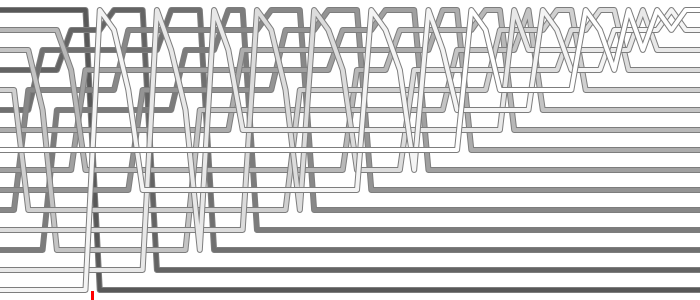
\includegraphics[height=45mm]{slike/Heap.png}
    \end{center}
    \vspace{-0.7cm}
    \caption[Urejanje s kopico]{Grafična predstavitev urejanja s kopico.}
    \label{fig:heapsortimage}
\end{figure}

V psevdokodi bi algoritem urejanja s kopico izgledal nekako tako:

\begin{algorithm}
  \caption{Urejanje s kopico}\label{algo:heapsort}
  \begin{algorithmic}[1]
    \Function{heapsort}{a, prvi, zadnji}
        \State \textsc{nakopiči}$(a, prvi, zadnji)$
        \While{$prvi < zadnji$}
            \Swap{a[prvi]}{a[zadnji]};
            \State $zadnji \gets zadnji - 1$
            \State \textsc{pogrezni}$(a, prvi, prvi, zadnji)$
        \EndWhile
    \EndFunction
    \\
    \Function{nakopiči}{a, prvi, zadnji}
        \State $zacetek \gets \lfloor(prvi + zadnji) / 2\rfloor - 1$
        \While{$zacetek \geq prvi$} \Comment{pogreznemo vse elemente, ki imajo otroke}
            \State $odmik \gets koren - prvi$
            \State \textsc{pogrezni}$(a, prvi, zacetek, zadnji)$
            \State $zadnji \gets zadnji - 1$
        \EndWhile
    \EndFunction
    \\
    \Function{pogrezni}{a, prvi, koren, zadnji}
        \State $odmik \gets koren - prvi$
        \While{$koren + odmik < zadnji$} \Comment{dokler ima koren vsaj enega otroka}
            \State $otrok \gets koren + odmik + 1$
            \State $zamenjava \gets koren$ \Comment{zapomnimo si, s čim je potrebno
            zamenjati koren}
            \If{$a[koren] < a[otrok]$} \Comment{če je otrok večji od korena}
            \State $zamenjava = otrok$\Comment{potem moramo zamenjati prvega otroka}
            \EndIf \Comment{če drugi otrok obstaja in je večji od trenutne zamenjave}
            \If{$otrok + 1 \leq zadnji \wedge zamenjava < a[otrok + 1]$}
                \State $zamenjava = otrok + 1$\Comment{potem zamenjamo njega}
            \EndIf
            \If{$zamenjava \neq koren$}
                \Swap{a[zam]}{a[koren]}
                \State $koren \gets zamenjava$
                \State $odmik \gets koren - prvi$
            \Else
                \State \Return 
            \EndIf
        \EndWhile
    \EndFunction
  \end{algorithmic}
\end{algorithm}

\subsubsubsection{Časovna in prostorska zahtevnost}
Časovna zahtevnost je v najboljšem, povprečnem in najslabšem primeru $O(n\log_2 n)$.

Prostorska zahtevnost je v vsakem primeru $O(1)$, saj je kopica predstavljena kar v
polju, ki ga urejamo, in ker se vse premene dogajajo na mestu.

Čas izvajanja urejanja s kopico je neodvisen od morebitne urejenosti podatkov v polju,
kot lahko razberemo iz časovne zahtevnosti. Zaradi dokaj zapletenega postopka sortiranja,
na manjših poljih ni tako uspešen, je pa čedalje bolj uspešen, ko se dolžina polja
povečuje.

\subsubsection{Urejanje z zlivanjem}
\label{chapter:mergesort}
Urejanje z zlivanjem (\emph{angl.} merge sort) je primerjalni sortirni algoritem, 
zgrajen na principu deli in vladaj. Razvil ga je John von Neumann leta 1945.
Urejanje z zlivanjem uporablja idejo, da je v sortirano polje hitreje združiti dve že
sortirani polji, kot pa dve še ne sortirani. 
Algoritem urejanja z zlivanjem ureja tako:
\begin{enumerate}
  \item če je polje dolgo 0 ali 1 je že sortirano, če ne:
  \item razdeli polje v dve približno enako dolgi podpolji
  \item sortiraj podpolji 
  \item združi podpolji nazaj v celotno sortirano polje.
\end{enumerate}

Algoritem je grafično prikazan na sliki \ref{fig:mergesortimage} na primeru sedmih
naključno izbranih števil.
Vsaka vrstica števil predstavlja svojo globino rekurzije, vse dokler niso polja dolga le
po en element. Nato se začne izvajati četrta točka algoritma, ponazorjena z vrsticami
nižje od črtkane črte, ki združi podpolja v sortirano polje.

\begin{figure}[h]
    \begin{center}
        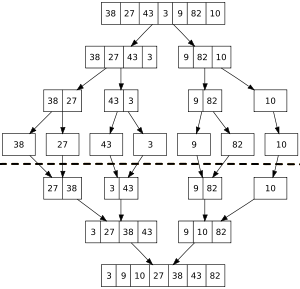
\includegraphics[height=50mm]{slike/merge_sort.png}
    \end{center}
    \vspace{-0.7cm}
    \caption[Urejanje z zlivanjem]{Grafična predstavitev urejanja z zlivanjem.}
    \label{fig:mergesortimage}
\end{figure}

V psevdokodi je urejanje z zlivanjem zapisano kot algoritem \ref{algo:mergesort}. 

\begin{algorithm}
  \caption{Urejanje z zlivanjem}\label{algo:mergesort}
  \begin{algorithmic}[1]
    \Function{mergesort}{a, prvi, zadnji}
        \If{$zadnji - prvi < 2$} \Return \EndIf
        \State $srednji \gets \lfloor(prvi + zadnji) / 2\rfloor$
        \State \textsc{mergesort}$(a, prvi, srednji)$
        \State \textsc{mergesort}$(a, srednji + 1, zadnji)$
        \State \textsc{merge}$(a, prvi, srednji, zadnji)$
    \EndFunction
    \\
    \Function{merge}{a, prvi, srednji, zadnji}
        \State $i \gets prvi$
        \State $j \gets srednji$
        \State $rezultat = [\ ]$ \Comment{Naredimo prazno polje rezultat}
        \While{$i < srednji \wedge j < zadnji$}
            \If{$a[i] < a[j]$}
                \State $rezultat.append(a[i])$ \Comment{Dodamo a[i] v polje rezultat}
                \State $i \gets i + 1$
            \Else
                \State $rezultat.append(a[j])$ \Comment{Dodamo a[j] v polje rezultat}
                \State $j \gets j + 1$
            \EndIf
        \EndWhile
        \While{$i < srednji$}
            \State $rezultat.append(a[i])$ \Comment{Dodamo a[i] v polje rezultat}
        \EndWhile
        \While{$j < srednji$}
            \State $rezultat.append(a[j])$ \Comment{Dodamo a[j] v polje rezultat}
        \EndWhile
    \EndFunction
  \end{algorithmic}
\end{algorithm}

\subsubsubsection{Časovna in prostorska zahtevnost}
Časovna zahtevnost je v najboljšem, povprečnem in najslabšem primeru 
$O(n\log_2 n)$. Časovna zahtevnost urejanja z zlivanjem ni odvisna od
morebitne že delne urejenosti ali neurejenosti podatkov v polju. 

Prostorska zahtevnost je v vsakem primeru $O(n)$. % ker O(n + log n)

V praksi je urejanje z zlivanjem najbolj učinkovito na
sekvenčnih medijih, kot na primer tračnih enotah, ali na podatkovnih strukturah, ki nimajo hitrega
neposrednega dostopa do nekega elementa z njegovim indeksom, kot na primer povezani seznami.

\subsection{Nameni in cilji}
\subsection{Hipoteze}
\begin{enumerate}
  \item Kompoziten algoritem se obnese boljše na različnih tipih podatkov kot vsak
    posamezen algoritem.
    % kaj pa kakšna da bo beatov build-in sort
\end{enumerate}
\section{Metode dela}
Za preverjanje hipotez(e) sem si izbral eksperiment. Hipotez(o/e) je z njim najlažje
potrditi ali ovreči, drugih virov na to temo pa ni v izobilju. Pri pripravi eksperimenta
sem potreboval tudi nekaj sekundarnih virov. Za izvedbo eksperimenta sem implementiral vse 
v teoretičnem delu opisane sortirne algoritme. Za implementacijo sem si izbral programski 
jezik C++, predvsem zato, ker se program prevede v strojno kodo, nad katero ima programer
veliko nadzora. Zmožen je optimizacije na najnižji ravni, medtem ko je pisanje kode kljub
temu nezahtevno opravilo, kot pri drugih programskih jezikih tretje generacije.

\subsection{Implementacija sortirnih algoritmov}
\label{chapter:sortimplementation}
Vsak izmed sortirnih algoritmov je implementiran kot funkcija z dvema parametroma.
Vsaka funkcija sprejme dva iteratorja z naključnim dostopom (\emph{Random Access
Iterator} ali kar \emph{RAI}),
ki kažeta na prvi element, ki ga sortiramo, in na prvi element za tistim, ki ga sortiramo
zadnjega. Slednji je lahko neveljaven v polju (kaže preko njegovega konca).
Tako obliko funkcij sem si izbral predvsem zato, ker je v skladu z zapisom, ki ga uporablja
C++-ova knjižnica \emph{algorithm}. Drugi razlog je, da s tem zapisom dosežemo minimalno število
parametrov pri želeni funkcionalnosti. Če bi želeli le en parameter, bi bilo to
izvedljivo, vendar bi se morali odpovedati zmožnosti, da lahko sedaj uredimo le željeni
del polja. V primeru zgolj enega parametra to ne bi bilo možno, vedno bi se
urejalo celotno polje.

Vsak sortirni algoritem, ki sem ga implementiral, ureja zgolj z uporabo operatorja $<$
(``je manjše''), ki se obnaša enako kot operator linearne urejenosti $\leq$. Vsak
algoritem je definiran kot funkcija tipa \emph{void}, kar pomeni, da ne vrne ničesar in
torej spremeni vrstni red elementov polja, ki ji ga podamo.

\subsection{Implementacija kompozitnega sortirnega algoritma}
\label{chapter:tweaksort}
Ker so sortirni algoritmi vsak zase dobri na zgolj nekaterih dolžinah polj in se pri tej
lastnosti razlikujejo, nas to privede do zamisli, da bi pri dani dolžini $n$ uporabili tisti
sortirni algoritem, ki je pri tem $n$ najboljši. Torej moramo vedeti, pri katerem $n$ je
potrebno uporabiti kateri sortirni algoritem, kar pa si bomo morali zapomniti. V ta
namen sem definiral tip $conf\_t$, v katerem je shranjena konfiguracija kompozitnega
sortirnega algoritma. 

Konfiguracija pove, kateri sortirni algoritem naj se uporablja pri
katerem $n$. Konfiguracijo se lahko predstavi kot niz znakov z zelo preprostimi
pravili. To je zaželeno predvsem zato, ker je konfiguracija namenjena temu, da je trajna
in berljiva in je namenjena temu, da si jo uporabnik zapomni. Ker je predstavljena kot niz
znakov, jo lahko tudi zapiše v datoteko in jo po želji tudi spremeni.

Kompozitni sortirni algoritem torej vedno uporabi tisti sortirni algoritem, ki je zapisan
v konfiguraciji za trenutni $n$. Tako spremenjen algoritem za urejanje, bi torej vhodno
polje vedno uredil s čimbolj optimalnim sortirnim algoritmom (če bi bilo tako seveda
zapisano v konfiguraciji). Vendar imajo nekateri algoritmi za urejanje zaradi metode deli in vladaj,
ki jo uporabljajo pri urejanju, še to lepo lastnost, da polja delijo na manjša polja. Za
ta manjša polja pa lahko spet pogledamo v konfiguracijo, kateri sortirni algoritem je
najbolj zaželen in podpolje uredimo z le-tem. To nam prinese možnost veliko hitrejšega
urejanja polj, saj se lahko odločimo, kateri sortirni algoritem bomo
uporabili, ne le za vhodno polje, temveč tudi za nekatera podpolja, ki jih ustvarijo
sortirni algoritmi, kot na primer hitro urejanje ali urejanje z zlivanjem.

Kompozitni sortirni algoritem mora torej pri svoji implementaciji poleg dveh 
iteratorjev z naključnim dostopom sprejeti tudi konfiguracijo. Procedura \emph{sort},
ki predstavlja kompozitni sortirni algoritem deluje enako kot algoritem
\ref{algo:tweaksort}. 

\begin{algorithm}
  \caption{Kompozitni sortirni algoritem}\label{algo:tweaksort}
  \begin{algorithmic}[1]
    \Function{sort}{prvi, zadnji, conf}
        \State $n \gets zadnji - prvi$
        \State $algoritem \gets$ \textsc{najdi\_pravi\_algoritem}$(n, conf)$
        \State \label{line:usealgo}Sortiraj z $algoritmom$.
    \EndFunction
  \end{algorithmic}
\end{algorithm}

Če v $algoritmu$, ki ga kličemo pri algoritmu \ref{algo:tweaksort} na vrstici
\ref{line:usealgo}, pride do rekurzivnega klica, naj kliče funkcijo \emph{sort} namesto
samega sebe.

Potrebno je bilo tudi rahlo spremeniti ostale sortirne algoritme, da namesto rekurzivnega
klica samega sebe kličejo proceduro \emph{sort} in tako pustijo, da se manjša polja morda uredijo z
drugim sortirnim algoritmom ter prispevajo k bolj učinkovitemu urejanju celotnega polja. Da pa
sortirni algoritmi sploh lahko kličejo glavno proceduro \emph{sort}, morajo kot
parameter prejeti tudi konfiguracijo, ki jo na koncu podajo nazaj proceduri \emph{sort}.

Funkcija \emph{najdi\_pravi\_algoritem}, ki jo kliče procedura \emph{sort}, se mora ob vsakem klicu odločiti, kateri
algoritem naj uporabi. Po celi konfiguraciji mora torej poiskati, kateri sortirni algoritem
naj uporabi, kar običajno terja časovno zahtevnost
$O(n)$, kjer je $n$ število vnosov v konfiguracijo. Ker pa mora biti podana konfiguracija
smiselna, mora biti urejena naraščajoče. Torej lahko želeni dolžini priredimo sortirni
algoritem v logaritemskem času, in ne v linearnem, z uporabo bisekcije. To je velika
izboljšava še posebej za dolge konfiguracije.

Da je konfiguracija smiselna mora biti sestavljena iz zaporedij oblike
\[ :sort\ \konfarrow\ \check{s}tevilo; \]

``sort'' pove, kateri sortirni algoritem naj se uporablja na katerih poljih. Črka, ki
prestavlja posamezen algoritem, je prva črka njegovega angleškega imena.

``število'' predstavlja katerokoli možno dolžino polja, ki ga sortiramo. Torej je lahko
katerokoli nenegativno število. Dovoljeno je tudi število $-1$, ki predstavlja neskončno
($\infty$).

Zadostiti pa mora tudi dvema pogojema:
\begin{enumerate}
  \item števila morajo biti urejena naraščajoče in
  \item zadnje in samo zadnje število mora biti $-1$.
\end{enumerate}
S tema dvema pogojema dosežemo, da se za vse možne dolžine polj enolično
določi, kateri ``sort'' naj se uporablja, kar je tudi namen konfiguracije.

V nadaljevanju naloge bom pri vseh primerih konfiguracij zaradi večje preglednosti 
namesto ``\konfarrow'' pisal ``\lra''. \\

Primer smiselne konfiguracije:
\[ :i \lra 20;:h \lra 45;:i \lra 123;:q \lra 7925;:m \lra -1; \]
Konfiguracija upošteva vsa slovnična pravila.
Števila so urejena naraščajoče in samo zadnje število je $-1$. Ta konfiguracija je torej
pravilna in smiselna. Konfiguracija pove, da naj se polja, katerih dolžine so iz intervala $\left[0,
20\right]$ ureja z vstavljanjem, polja z dolžinami iz intervala $\left(20, 45\right]$ naj
se ureja s kopico, polja, ki imajo dolžine na intervalu $\left(45, 123\right]$ zopet z vstavljanjem,
polja z dolžinami na intervalu $\left(123, 7925\right]$ s porazdelitvami, polja, katerih dolžine pa so iz
intervala $\left(7925, \infty\right)$ oziroma tista, katerih dolžine so večje od 7925
pa naj se ureja z zlivanjem. Tako je za prav vse možne dolžine enolično določeno, kateri
sortirni algoritem naj bo uporabljen.

Oglejmo si še nekaj realnih primerov, dobljenih za različne tipe podatkov.
\[ :i \lra 142;:q \lra -1;\]
\[ :m \lra -1; \]
Tudi ta dva primera sta smiselna. V prvem vidimo da naj se uporablja urejanje z
vstavljanjem, če je dolžina polja manjša ali enaka 142, sicer naj se uporablja hitro
urejanje. Pri drugem primeru, ki je tudi eden izmed najkrajših možnih primerov
konfiguracije, se uporablja samo urejanje z zlivanjem.\\

Primer nesmiselne konfiguracije:
\[ :i \lra 60;:h \lra 45;:i \lra 145;:q \lra 7925;:m \lra 33456;:q \lra -1 \]
Konfiguracija sicer upošteva vsa slovnična pravila, vendar je nesmiselna. Prva napaka je,
da števila niso urejena naraščajoče, s tem torej ni zagotovljena enolična določenost,
kateri sortirni algoritem naj se uporabi. V konfiguraciji piše, da naj se polja z
dolžinami od 0 do 60 urejajo z vstavljanjem, tista z dolžinami od 60 do 45 pa s kopico.
Torej ni enolično definirano, s katerim algoritmom naj uredimo polja dolžine 52, na primer. 

Še nekaj primerov nesmiselnih konfiguracij:
\[ 50 \lra i:;q \lra -1; \]
\[ :i \lra 22;:q \lra 450; \]
\[ :s \lra 234;:q \lra -1;: m \lra 3456; \]
Pri prvem primeru je konfiguracija ne le nesmiselna temveč tudi nepravilno oblikovana.
Pri drugem primeru je nesmiselno to, da konfiguracija ne vsebuje števila $-1$, in tako ne
definira kateri algoritem naj se uporablja za polja z dolžinami večjimi od 450.
Pri zadnjem je nesmiselno to, da število $-1$, ni na koncu, torej so
vsi vnosi za tem nepotrebni.

%Vsak \ntm{vnos} pove, do katere dolžine (vključno z napisano), naj se uporablja kateri sortirni
%algoritem. Začetek uporabe tega sortirnega algoritma pa označuje število, pri katerem se
%uporaba prejšnjega zaključi. Prvi sortirni algoritem -- tisti, ki ga definira prvi
%\ntm{vnos} -- in edini, ki nima predhodnika, se začne uporabljati pri 0, spodnji meji veljavnih dolžin
%polj (negativne dolžine ne obstajajo). Ker se uporaba nekega sortirnega algoritma začne
%tam, kjer se uporaba prejšnjega konča, je tako za vse dolžine polj definirano, kateri
%algoritem naj se uporabi, če le upoštevamo, da se algoritem, ki ga določa zadnji vnos,
%uporablja do neskončnosti. Torej mora biti pri zadnjem vnosu in samo pri zadnjem vnosu 
%\ntm{število} nujno enako $-1$, da je konfiguracija smiselna. To je potreben pogoj, ker obstaja možnost, da bi
%kompozitni sortirni algoritem dobil polje, ki je daljše od njegovega zadnjega, največjega
%vnosa v konfiguraciji in torej ne bi znal urediti polja, ker ne bi vedel, kateri sortirni
%algoritem naj uporabi. Ker pa je zadnje \ntm{število} vedno enako $-1$, ne more biti nobeno
%polje izven mej, ki jih kompozitni algoritem podpira.
%Pogoj za smiselnost konfiguracije je tudi, da so števila urejena naraščajoče, saj se le tako lahko
%enolično določi spodnje meje uporabe posameznih sortirnih algoritmov. 

Ker se procedura \emph{sort} uporablja v knjižnici, potebujemo tudi pretvornik
konfiguracije v niz znakov in obratno. Zaradi tega je potrebno definirati slovnico
konfiguacije. Tolmač konfiguracije iz niza znakov v \emph{conf\_t} sicer dopušča bolj ohlapna pravila, kot so
definirana v slovnici, vendar odsvetujem uporabo ohlapnejšega zapisa.

Formalna definicija slovnice konfiguracije v notaciji
BNF\footnote{Backus--Naur Form,\\ vir: \url{http://www.cui.unige.ch/db-research/Enseignement/analyseinfo/AboutBNF.html}} 
je sledeča: % kaj več o BNF ? Vsaj uvod v teoriji
\\
\begin{BNF} %% zakaj maš ti kle ~BNF
  \begin{align*}
    \abnf{sort}{\q{i} \ali \q{s} \ali \q{q} \ali \q{h} \ali \q{m}}\\
    \abnf{število}{\in \N \ali \q{-1}} \\
    \abnf{vnos}{\q{:}\ntm{sort}\q{\mbox{--}\ \mbox{--}\ \mbox{$>$}}\ntm{število}\q{;}}\\
    \abnf{konfiguracija}{\ntm{vnos} | \ntm{konfiguracija}\ntm{vnos}}
  \end{align*}
\end{BNF}

\subsection{Iskanje optimalne konfiguracije}
\label{chapter:optimalconf}
Za hitrost procedure \emph{sort} je bistvena konfiguracija.
Torej je iskanje optimalnega kompozitnega sortirnega algoritma pravzaprav iskanje optimalne
konfiguracije zanj. Ker uporabnik ne ve, katera konfiguracija je optimalna, sem napisal
funkcijo, ki to ugotovi. 

Glavna ideja je, da lahko
dva kompozitna sortirna algoritma lahko primerjamo po času izvajanja. Tisti, ki porabi manj
časa, je boljši pri trenutni dolžini polja, ki sta ga urejala.
S tem smo definirali relacijo $a$ je $n$ boljši od $b$:
\[ a \leq_n b \Leftrightarrow a\ \text{je v povprečju na poljih dolžine $n$ boljši
od}\ b.\]
Tako lahko problem rešimo kar s požrešno metodo: 
pri posamezni dolžini ugotovimo, kateri algoritem je najboljši in to vnesemo
v konfiguracijo. Glavni podatek, ki nam ga poda uporabnik, je meja učenja. To je zadnja
dolžina, za katero bo algoritem še iskal optimalno konfiguracijo. Od te dolžine naprej
konfiguracija ni več nujno optimalna. Seveda v konfiguracijo pišemo le, če pride do 
spremembe na vodilnem mestu. Algoritem za iskanje najboljše konfiguracije je opisan v
sledečih točkah.
\begin{enumerate}
  \item \label{step:init}Preveri, katera od začetnih možnosti konfiguracij je najboljša in
    si jo zapomni, imenujmo jo $za\check{c}etna$. Začetne možnosti konfiguracij so:
    ``$:i \lra -1;$'', ``$:q \lra -1;$'', ``$:h \lra -1;$'',
    ``$:m \lra -1;$'', ``$:s \lra -1;$'', torej ko sortirni algoritem še ni kompoziten.
  \item \label{step:start}Povečaj $n$, trenutno dolžino polja, za neko razdaljo. Imenujmo
    jo $razdalja$. Povečaj tudi $razdaljo$, za neko konstantno vrednost, imenovano
    $pospe\check{s}ek$.
  \item Preveri, katera od konfiguracij je pri tem $n$ najboljša.
  \item \label{step:check}Če je enaka kot $za\check{c}etna$, ponovi korake od \ref{step:start} 
    naprej. Če se razlikujeta, si v končno konfiguracijo dodaj zapis, da je
    trenuten kompozitni sortirni algoritem najboljši do $n - razdalja$.
  \item Če je $n$ večji od $M$, meje učenja, potem spremeni zadnji zapis v konfiguraciji
    tako, da bo zadnji sortirni algoritem sortiral vsa polja, torej ga nastavi na $-1$.
    Nato končaj.
  \item Če je $n$ manjši od $M$, potem $n$ zmanjšaj za trenutno razdaljo, saj
    tako razdaljo nastavimo na zadnjo vrednost, ko vemo, kateri algoritem je bil
    najboljši.
  \item Naredi nove morebitne konfiguracije, tako, da trenutni končni konfiguraciji dodaš
    vsako izmed začetnih konfiguracij iz koraka \ref{step:init}.
  \item Ponovi korake od \ref{step:start} naprej.
\end{enumerate}

Ažman bo z veseljem dokazal, da algoritem deluje pravilno. \smiley\  
Jaz bom zraven in se bom čudil in trudil razumeti, tako, da bom kasneje znal razložiti
celoten postopek. \blacksmiley

Funkcija, ki implementira algoritem za iskanje optimalne konfiguracije 
se imenuje \emph{learn} in je definirana tako:

%% problem z & spet

\begin{lstlisting}
    conf_t learn(const size_t M, 
                 const Compare<container_t>& cmp);
\end{lstlisting}

\begin{itemize}
  \item Parameter $M$ predstavlja mejo učenja. Parameter je
    konstanten, funkcija ga ne sme spreminjati. M ima tip \emph{size\_t}, kar je najmanj 32
    bitno nenegativno celo število, torej predstavlja ravno tista števila, ki so veljavne
    dolžine polj.
  \item Parameter $cmp$ predstavlja objekt tipa $Compare$, ki pomaga pri primerjanju
    različnih sortirnih metod. Parameter je konstanten, funkcija ga ne spreminja.
    Parameter je podan kot referenca (označeno z \&), kar pomeni, da se ob klicu funkcije
    ne bo kopirala njegova vrednost, ampak se bo podal kar točno ta objekt. To je precej
    pomembno, saj je pričakovano, da je ta parameter precej velik in je zaradi tega
    kopiranje neprimerno. 
\end{itemize}

Objekt $Compare$ je definiran tako:
\begin{lstlisting}
    Compare(const size_t iterations, 
            const size_t limit, 
            const double acceleration, 
            const container_t& data);
\end{lstlisting}


\begin{itemize}
  \item Parameter $iterations$ pomeni, koliko iteracij posamezne sortirne metode bo naredil
    program, preden zabeleži njen rezultat. Večje kot je to število, bolj natančne so
    meritve.
  \item Parameter $limit$ pomeni število elementov, ki jih lahko hranimo v pomnilniku.
    Večje ko je to število, hitrejši bo program. Mora biti najmanj $M$. Program bo v
    pomnilniku hranil največ $iterations \cdot M$ elementov, tudi če je dovoljen limit večji od
    tega.
  \item Parameter $acceleration$ pomeni pospešek povečevanja dolžine polj, ki jih bo
    program sortiral. Skok na naslednjo dolžino se bo vsakič povečal za vrednost tega
    parametra. Primer: če je $acceleration$ enak 2, se bo program učil na poljih dolžine
    $1, 2, 5, 10, 17, 26$. Razdalja med elementi se vsakič poveča za 2. Nuno mora biti
    pozitiven ali enak $0$.
  \item Parameter $data$ predstavlja podatke, iz katerih bo program jemal naključne
    elemente za polja, ki jih bo sortiral. Polja bodo enakega tipa kot $data$, saj ima
    lahko tip podatkovne strukture velik vpliv na hitrost algoritmov. Podatki naj
    predstavljajo čim bolj tipične podatke, ki bodo kasneje sortirani, saj bodo tako
    rezultati boljši. Ta parameter je podan kot referenca, s tem preprečimo kopiranje
    tega običajno velikega parametra v pomnilniku.
\end{itemize}
Vsi parametri so podani kot konstantni, saj se znotraj funkcije ne smejo spreminjati. 

\subsection{Merjenje časa izvajanja posameznih algoritmov}
Merjenje časa izvajanja posameznih sortirnih algoritmov je pravzaprav edini način za
primerjanje njihove uspešnosti in zato temu delu naloge namenil veliko pozornosti.

Parametri, ki nam jih poda uporabnik, so v definirani v poglavju
\ref{chapter:optimalconf}. Za merjenje časa sta pomembna le dva, to sta $iterations$ in
$limit$. Parameter, ki ga še potrebujemo, pa je dolžina polja, ki ga bo sortirni algoritem
urejal, imenujmo ga $n$.

Najbolj naiven algoritem za merjenje časa bi verjetno izgledal podobno naslednjemu. 
Naredimo polje dolžine $n$ in si zapomnimo trenuten čas. Premešamo polje in ga
uredimo z želenih algoritmom. Ponovimo zadnje dva koraka tolikokrat, da je število
ponovitev enako številu, ki ga je podal uporabnik. Nato si spet zapomnimo čas in kvocient
med razliko in številom iteracij je naš željeni rezultat.

Glavna napaka zgornjega algoritma je v tem, da v celoten čas šteje tudi tisti čas, ko
mešamo polje, ne le tistega, ko se polje sortira. To bi lahko odpravili tako, da bi pred
in po vsakem urejanju zabeležili čas, čase nato sešteli in jih delili z številom iteracij,
vendar to ne bi bilo dovolj natančno, saj merjenje tako kratkih časovnih intervalov,
še posebej, ko se sortirajo kratka polja, enostavno ni dovolj natančno, da bi bilo
statistično zanesljivo. Zaželeno je torej, da se meri zgolj čas, ki ga algoritem porabi za
urejanje polja, poleg tega pa je zaželeno tudi, da bi povečali natančnost meritve, da se mora
pri določeni dolžini polja opraviti več urejanj hkrati, ki jim izmerimo skupni čas, iz katerih se nato izračuna povprečno
vrednost. Ker želimo, da merimo zgolj čas, ko algoritem ureja, moramo pred tem shraniti
premešana polja shraniti v pomnilnik. Tu nastopi parameter $limit$, ki pove, koliko
elementov smemo imeti v pomnilniku. Večji ko je limit, več meritev se bo izvedlo naenkrat,
in rezultat bo bolj natančen in statistično zanesljiv.

Čas izvajanja bom meril z funkcijo \emph{clock\_gettime}, ki ima od vseh znanih
funkcij največjo natančnost (meri do nanosekunde natančno), kar je dovolj
za naše potrebe.

Algoritem, ki meri čas posameznega algoritma je sledeč. Zapisan je v psevdokodi kot
algoritem \ref{algo:time}.

\begin{enumerate}
  \item Definirajmo spremenljivko $\check{c}as$ in $napredek$, ter ju nastavimo na 0
    (vrstica \ref{line:init}, algoritem \ref{algo:time}).
  \item \label{time:start} Ugotovimo, koliko polj si lahko pripravimo za testiranje. To je seveda odvisno od
    limita, ki nam ga je podal uporabnik. Pripravimo si največ $\lfloor limit/n \rfloor$
    polj, kjer je $n$ dolžina polja. Naj bo $k$ število polj, ki jih bomo morali
    pripraviti.
    Če pripravimo samo $k$ polj zagotovo ne bomo prebili limita uporabnika.
    Če pa je razlika med napredkom in želenim številom iteracij še manjša
    od $k$, potem si  moramo pripraviti le toliko polj, kot je še želenih iteracij.
    To naredi vrstica \ref{line:koliko}, kjer \textsc{min} predstavlja funkcijo, ki vrne
    manjšega od dveh parametrov.
  \item Pripravimo si želeno število polj. To naredi na vrstici
    \ref{line:polja} klicana funkcija \textsc{naredi\_naključna\_polja}. Njeno obnašanje
    je sledeče: naredi vektor polj, ki so enakega tipa kot tisto, ki nam ga je podal 
    uporabnik kot parameter $data$. Nato polja napolni z
    naključnimi elementi iz njegovega podanega polja. Z izbiro naključnih elementov in ne 
    naključnih rezin preprečimo, da bi morda dobili drugačne nezaželene rezultate. To bi
    se lahko zgodilo če bi uporabnik na primer pozabil zmešati polje, preden ga poda, in bi se, če bi jemali 
    zolj rezine, vedno sortirala še urejena polja, kar bi dalo precej drugačne rezultate 
    kot sicer.
  \item Zapomnimo si trenuten čas (vrstica \ref{line:getstarttime}), nato uredimo vsa predpripravljena polja z želenim
    sortirnim algoritmom (vrstice \ref{line:beginsortfor} -- \ref{line:endsortfor}) in si
    nato spet zapomnimo čas (vrstica \ref{line:getendtime}.
  \item Razliko v času prištejemo spremenljivki $\check{c}as$ in povečamo napredek za $k$. 
  \item Če je napredek večji ali enak želenemu številu ponovitev, končaj. 
    Drugače ponovi vse korake od \ref{time:start} naprej. To ponavljanje je prikazano v
    \emph{repeat} zanki med vrsticama \ref{line:repeattimestart} in
    \ref{line:repeattimeend}.
  \item Deli $\check{c}as$ s številom iteracij, ki so bile izvedene (tako dobimo čas
    izvajanja za urejanje enega samega polja) in to je iskana vrednost, ki jo vrnemo na
    vrstici \ref{line:returnaverage}.
\end{enumerate}

\begin{algorithm}
  \caption{Merjenje časa}\label{algo:time}
  \begin{algorithmic}[1]
    \State \label{line:init} $\check{c}as \gets napredek \gets 0$
    \Repeat \label{line:repeattimestart}
      \State \label{line:koliko} $koliko \gets $\textsc{min}$(\lfloor limit / n \rfloor, iteracije - napredek)$
      \State \label{line:polja} $polja \gets $\textsc{naredi\_nalkjučna\_polja}$(koliko, data)$
      \State \label{line:getstarttime} $start \gets $\textsc{dobi\_čas}$()$
      \For{i}{0}{koliko} \label{line:beginsortfor}
        \State Uredimo polje $polja[i]$ z želenih algoritmom
      \EndFor \label{line:endsortfor}
      \State \label{line:getendtime} $stop \gets $\textsc{dobi\_čas}$()$
      \State $\check{c}as \gets \check{c}as + stop - start$
      \State $napredek \gets napredek + koliko$
    \Until{$napredek \geq iteracije$} \label{line:repeattimeend} \\
    \Return \label{line:returnaverage}$\check{c}as / iteracije$
  \end{algorithmic}
\end{algorithm}
Tako merimo zgolj čas, ko algoritmi urejajo, hkrati pa se držimo limita v pomnilniku, ki
nam ga je določil uporabnik. Časa, ko ustvarjamo polja tako ne upoštevamo k rezultatu, kot
je tudi prav.

\section{Rezultati}
So obetavni.
\section{Ugotovitve in razprava}
\section{Sklep}
Potrdili smo hipotezo. Rezultate bi lahko izboljšali z bolj optimizirano implementacijo.
\section{Zaključek}
Zadeva je uporabna.
\section{Viri}
\subsection{Literatura}
\vspace{-1cm}
\begin{thebibliography}{99}
  \bibitem[KOZ86]{bib:koz86} {J. Kozak, \emph{Podatkovne strukture in algoritmi}. DMFA SRS, Ljubljana 1986. }
\end{thebibliography}
\subsection{Priloge}


\end{document}
% vim: spell spelllang=sl
